\documentclass{standalone}

%----------------------------------------------------------------------------------------------%
%                                 Packages and basic declarations
%----------------------------------------------------------------------------------------------%

\usepackage[utf8]{inputenc}
\usepackage{pgfplots}
\usepackage{tikz}


%----------------------------------------------------------------------------------------------%
%----------------------------------------------------------------------------------------------%
%                                            DOCUMENT STARTS
%----------------------------------------------------------------------------------------------%
%----------------------------------------------------------------------------------------------%

\begin{document}


%Tikz picture starts%

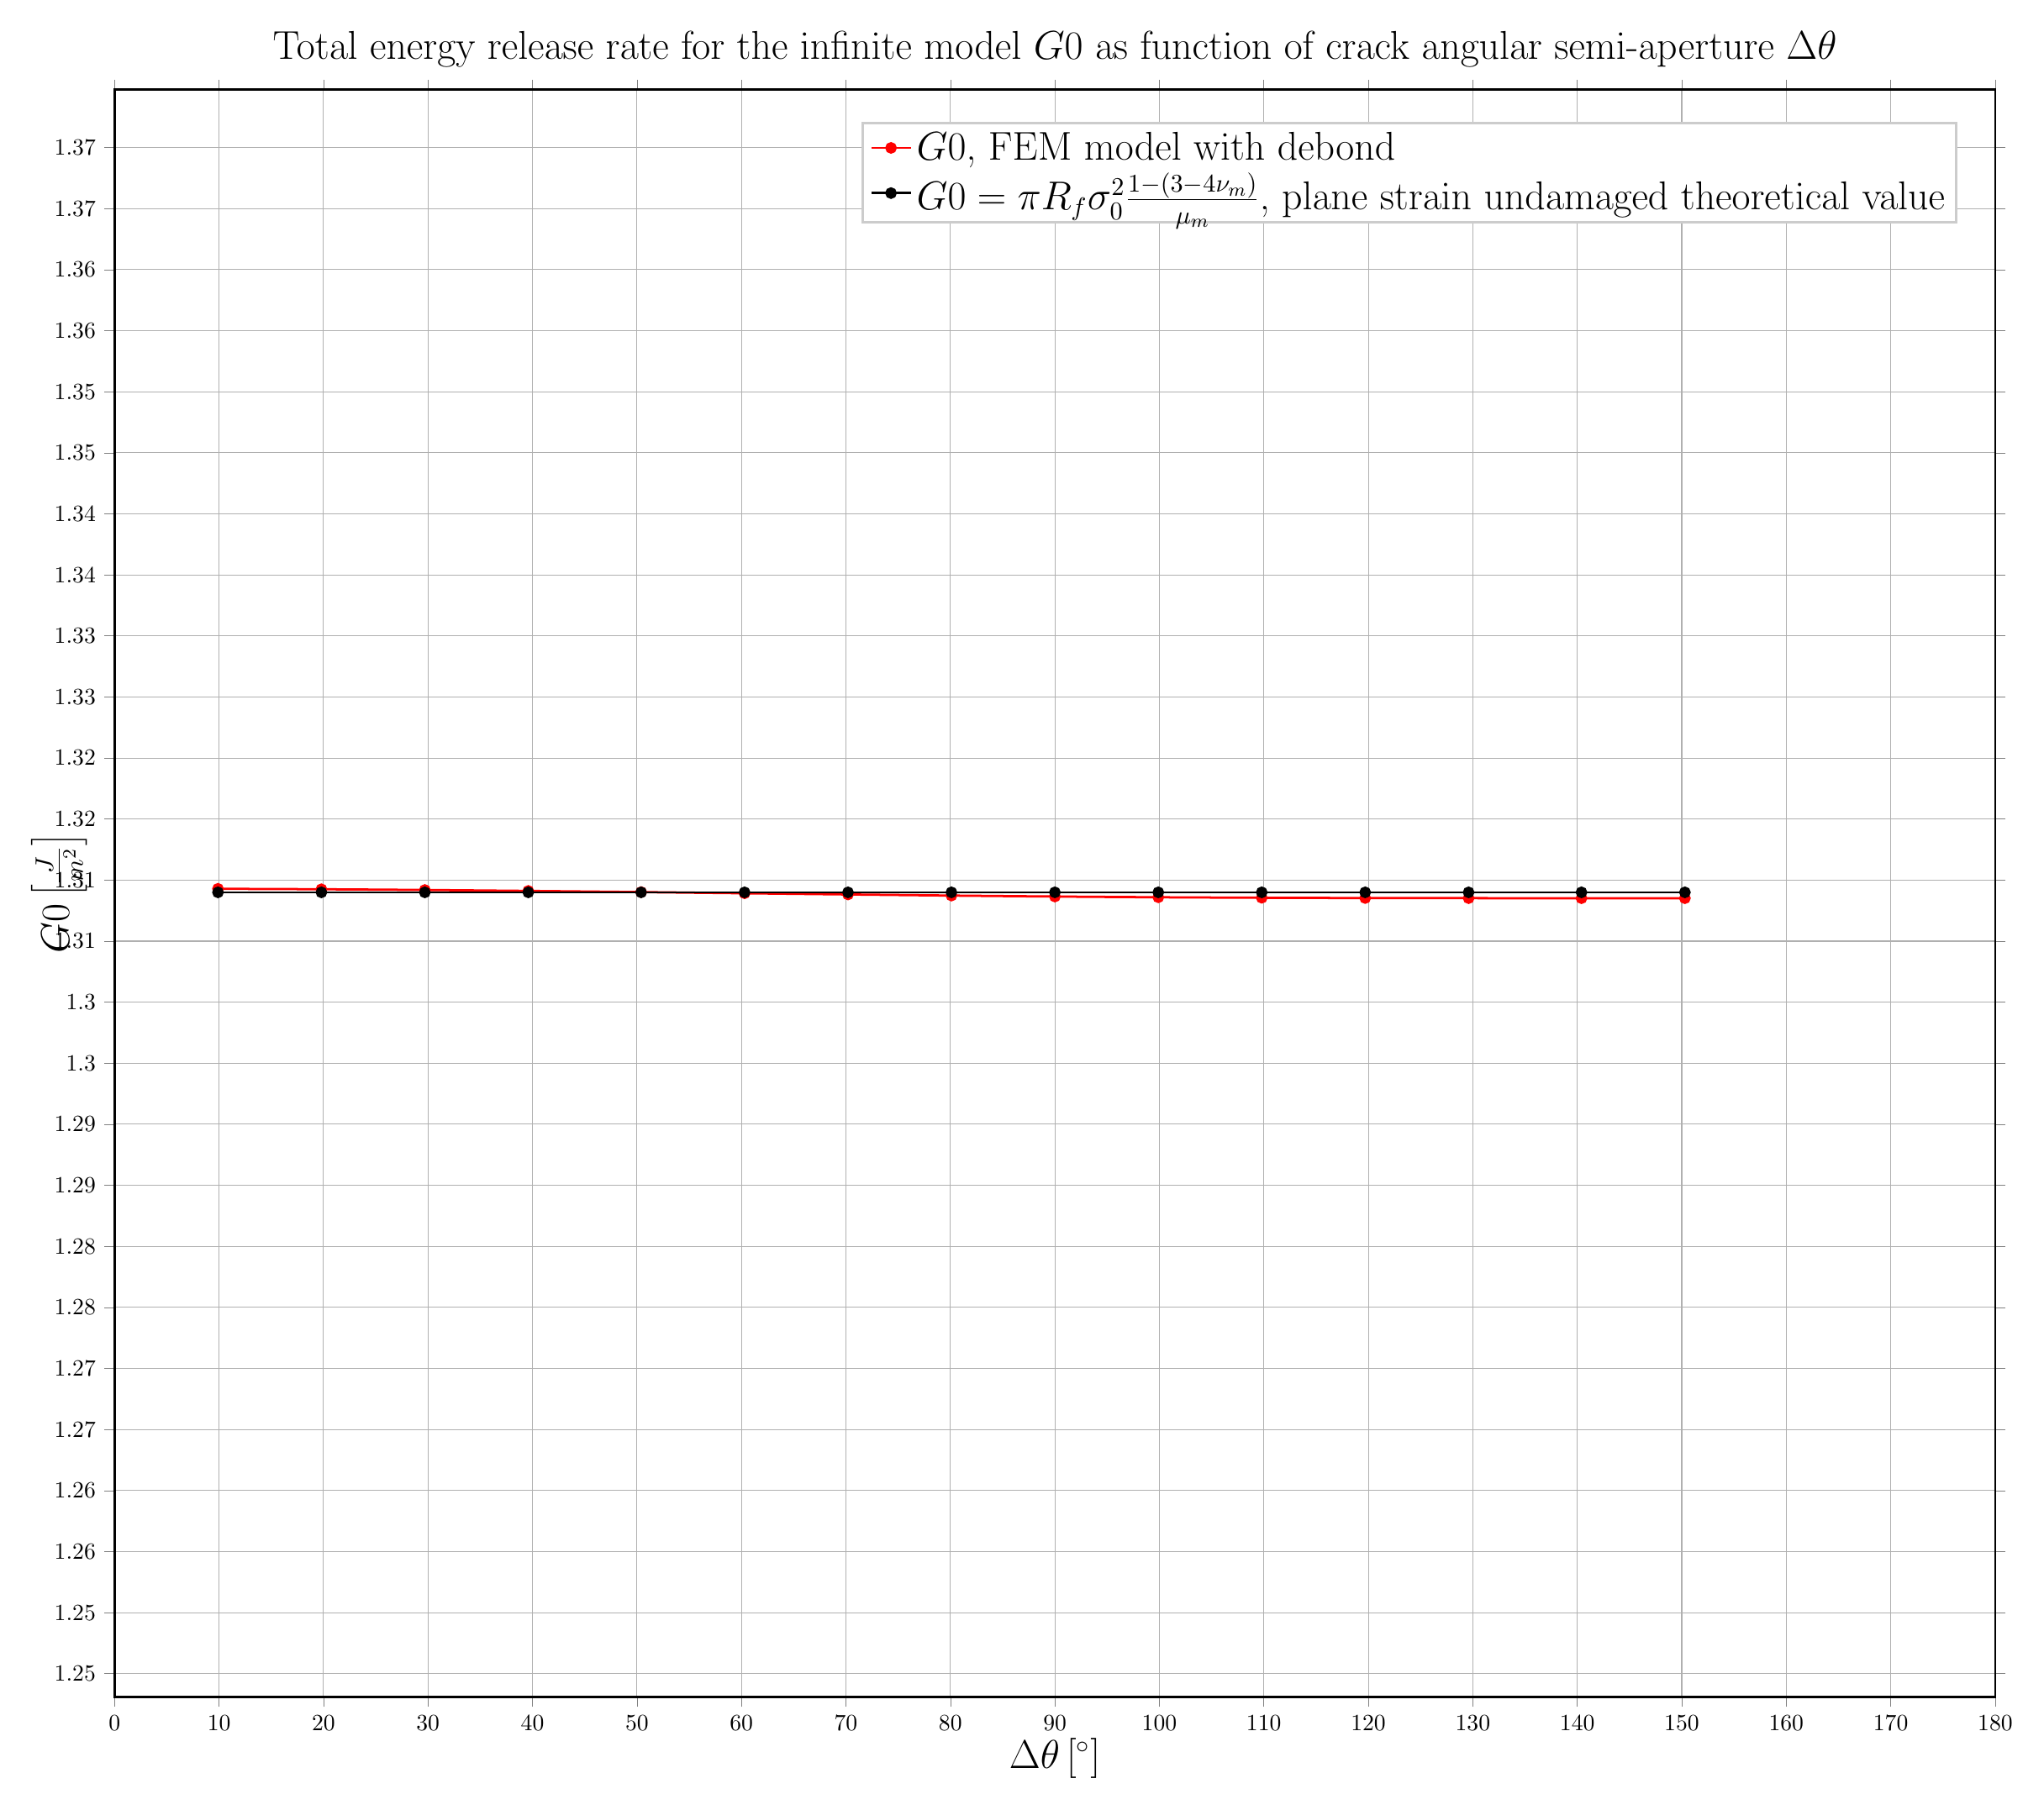
\begin{tikzpicture}

%Tikz axis starts%

\begin{axis}[width=30cm,
title={Total energy release rate for the infinite model $G0$ as function of crack angular semi-aperture  $\Delta\theta$},
title style={font=\fontsize{16}{8}\selectfont},
xlabel style={at={(axis description cs:0.5,-0.02)},anchor=north,font=\fontsize{16}{8}\selectfont},
ylabel style={at={(axis description cs:-0.01,.5)},anchor=south,font=\fontsize{16}{8}\selectfont},
xlabel={$\Delta\theta\left[^{\circ}\right]$},ylabel={$G0\left[\frac{J}{m^{2}}\right]$},
xmin=0.0,
xmax=180.0,
ymin=1.24309013433,
ymax=1.37475061464,
tick align=outside,
tick label style={font=\normalsize},
xtick={0.0,10.0,20.0,30.0,40.0,50.0,60.0,70.0,80.0,90.0,100.0,110.0,120.0,130.0,140.0,150.0,160.0,170.0,180.0},
xmajorgrids,
x grid style={lightgray!92.026143790849673!black},
ymajorgrids,
y grid style={lightgray!92.026143790849673!black},
line width=0.35mm,
legend style={draw=white!80.0!black,font=\fontsize{16}{12}\selectfont},
legend entries={{$G0$, FEM model with debond},{$G0=\pi R_{f}\sigma_{0}^{2}\frac{1-\left(3-4\nu_{m}\right)}{\mu_{m}}$, plane strain undamaged theoretical value}},
legend cell align={left}
]

\addplot[red,smooth,mark=*]
table{
9.90004415946 1.30928629966
19.800125885 1.30924907589
29.700111134 1.30919001949
39.5999409963 1.3091133622
50.4000580931 1.30901569299
60.2998879554 1.30891957465
70.1998714969 1.30882303152
80.0999574912 1.30873209786
90.0000025045 1.30865362217
99.9000475177 1.30859312945
109.800126682 1.30855253798
119.700103393 1.30852966515
129.599943501 1.30851975088
140.400057182 1.30851694993
150.29988363 1.30851676724
};

\addplot[black,smooth,mark=*]
table{
9.90004415946 1.308996939
19.800125885 1.308996939
29.700111134 1.308996939
39.5999409963 1.308996939
50.4000580931 1.308996939
60.2998879554 1.308996939
70.1998714969 1.308996939
80.0999574912 1.308996939
90.0000025045 1.308996939
99.9000475177 1.308996939
109.800126682 1.308996939
119.700103393 1.308996939
129.599943501 1.308996939
140.400057182 1.308996939
150.29988363 1.308996939
};

\end{axis}
%Tikz axis ends%


\end{tikzpicture}
%Tikz picture ends%


\end{document}

%----------------------------------------------------------------------------------------------%
%----------------------------------------------------------------------------------------------%
%                                            DOCUMENT ENDS
%----------------------------------------------------------------------------------------------%
%----------------------------------------------------------------------------------------------%

